\documentclass[conference]{IEEEtran}
\IEEEoverridecommandlockouts
% The preceding line is only needed to identify funding in the first footnote. If that is unneeded, please comment it out.
\usepackage{cite}
\usepackage{amsmath,amssymb,amsfonts}
\usepackage{algorithmic}
\usepackage{graphicx}
\usepackage{textcomp}
\usepackage{xcolor}
\usepackage{array}
\usepackage{multirow}
\def\BibTeX{{\rm B\kern-.05em{\sc i\kern-.025em b}\kern-.08em
    T\kern-.1667em\lower.7ex\hbox{E}\kern-.125emX}}
\begin{document}

\title{Analysis of Programming Students' Prompts to Identify Patterns of
Critical Thinking in Interactions with Generative AI \\
{\footnotesize \textsuperscript{*}Note: Sub-titles are not captured in Xplore and
should not be used}
\thanks{Identify applicable funding agency here. If none, delete this.}
}

\author{\IEEEauthorblockN{1\textsuperscript{st} Rodrigo Prestes Machado}
\IEEEauthorblockA{\textit{dept. Informática} \\
\textit{Instituto Federal do Rio Grande do Sul}\\
Porto Alegre, Brazil \\
0000-0003-0428-6387}
\and
\IEEEauthorblockN{2\textsuperscript{nd} Carlos Alario Hoyos}
\IEEEauthorblockA{\textit{Dep. Ingeniería Telemática} \\
\textit{Universidad Carlos III de Madrid}\\
Madrid, Spain \\
0000-0002-3082-0814}
\and
\IEEEauthorblockN{3\textsuperscript{rd} Carlos Delgado Kloos}
\IEEEauthorblockA{\textit{Dep. Ingeniería Telemática} \\
\textit{Universidad Carlos III de Madrid}\\
Madrid, Spain \\
0000-0003-4093-3705}
}

\maketitle

\begin{abstract}
This document is a model and instructions for \LaTeX.
This and the IEEEtran.cls file define the components of your paper [title, text, heads, etc.]. *CRITICAL: Do Not Use Symbols, Special Characters, Footnotes, 
or Math in Paper Title or Abstract.
\end{abstract}

\begin{IEEEkeywords}
component, formatting, style, styling, insert
\end{IEEEkeywords}

\section{Introduction}

%What is the problem to be solved?

Recent advancements in Generative Artificial Intelligence (GenAI) have opened
up new possibilities in education. In programming courses, students can utilize
GenAI tools to improve their understanding, receiving assistance, feedback, and
detailed explanations.

The study by Chan and Hu et al. \cite{chan23} revealed that both undergraduate
and postgraduate students exhibit positive attitudes toward the use of GenAI
in teaching and learning, noting that it enhances the depth of their thinking
and understanding. Additionally, a systematic review by Lo, Hew, and Jong
\cite{Lo24} demonstrated that students could effectively learn from ChatGPT,
leading to improved understanding and academic achievement. Cai et al.
\cite{cai23} further observed that ChatGPT enables students to regulate their
learning pace, promoting self-regulation.

In the other hand, researchers have concerns about the impact of these
tools on students. The systematic review of Vargas-Murillo et al.
\cite{Murillo23} indicated that ChatGPT use might lead to an overreliance on the
tool. Chan et al. \cite{chan23} also noted that this reliance could result in a
decrease in critical thinking, as students might make decisions based solely on
the information provided by ChatGPT.

The student's confidence is warranted, as shown by Puryear and Sprint
\cite{Puryear22}, who demonstrated that GitHub Copilot can generate solutions
for student assignments with accuracy rates ranging from 68\% to 95\%. However,
this raises concerns that students might rely too heavily on GenAI tools,
potentially neglecting a deeper understanding of the underlying concepts.
Cai et al. \cite{cai23} further identified overdependence and reduced
intellectual engagement as significant drawbacks of using ChatGPT in learning.

Regardless of teachers' preferences or beliefs, preliminary surveys by Dickey,
Bejarano, and Garg \cite{Dickey24} revealed that at least 54.5\% of students are
already using Generative AI (GenAI) for homework. This highlights the need to
understand how students are interacting with these tools and how they can be
used to enhance learning. Furthermore, a review by Lo, Hew, and Jong \cite{Lo24}
emphasized the necessity for extended studies and objective measures to gather
more robust evidence on the use of GenAI tools in education.

% Are there any existing solutions?

To deal with this issue, some researchers have proposed different pedagogical
strategies. Denny et al. \cite{Denny24} introduced the concept of \textit{Prompt
Problems}, where students solve programming exercises by formulating natural
language prompts. Prasad and Aamod \cite{Prasad24} proposed a self-regulated
learning framework using GenAI to solve programming problems. Lauren and Watta
\cite{Lauren23} explored the integration of generative AI with evidence-based
learning strategies in computer science and engineering courses.

% Which is the best?

Effective strategies are crucial to determinate the best approaches and training
educators to use GenAI tools effectively can be time-consuming and
resource-intensive. Therefore, understanding how students interact with these
tools is essential. By analyzing these interaction patterns, we can assess the
impact of GenAI tools on students' learning outcomes.
This knowledge can then be used to refine the design of GenAI tools, ensuring
they better support pedagogical strategies and enhance overall learning
experiences.

% What is its main limitation?

It is important to consider how GenAI tools affect students across different
demographic groups, knowledge areas, and levels of programming experience.
Understanding these variations can provide insights into the impact of GenAI
tools on their learning outcomes, helping to tailor educational approaches that
address the specific needs of diverse student populations.

% What do you hope to achieve?

This study aims to analyze the interactions between students and CharlieBot,
an ChatGPT-based bot developed by UC3M that leverages Retrieval-Augmented
Generation (RAG) to enhance its contextual understanding of Java programming.

\section{Background}

The paper \cite{Lo24} From the cognitive perspective, students were able to
learn from ChatGPT, which increased their understanding and achievement.
However, concerns were raised that the growing use of AI tools might lead to
a decline in critical thinking among students. Teachers and stakeholders should
continue to investigate pedagogical approaches that leverage ChatGPT to enhance
students' understanding and critical thinking. For example, teachers can
instruct students to fact-check and validate information produced by ChatGPT.




examined students from different demographic groups
using AI tools like ChatGPT, comparing perceptions and impacts
among these groups. The results showed that AI tools had a positive impact on
academic performance, especially for students with less prior experience.

\subsection{Critical Thinking}

Critical thinking is a fundamental skill for students to develop, as it enables
them to analyze, evaluate, and synthesize information. This skill is essential
for problem-solving and decision-making, making it a crucial aspect of
educational success, specifically in programming courses. However, the use of AI
tools like ChatGPT has raised concerns about the potential impact on students'
critical thinking abilities \cite{Vargas2023} \cite{cai23} \cite{chan23}.


In the other hand, the study of \cite{zhang24} suggested that incorporating
ChatGPT could stimulate students' critical thinking, probably because they
had to assess the correctness of ChatGPT's answers.

Regarding self-regulation, \cite{cai23} noted that ChatGPT allowed students to
regulate their learning pace.

\cite{wu24} found that ChatGPT-supported learning not only promoted students'
self-regulation but also increased their self-efficacy.


\subsection{CharlieBot}

CharlieBot is a ChatGPT-based bot that provides assistance to students in Java
programming courses at UC3M. The bot uses RAG(retrieval augmented generation) to
generate responses to student queries, providing explanations, code snippets,
and debugging help. The goal of CharlieBot is to support students in their
learning process by providing personalized assistance and feedback.


\begin{table*}[htbp]
\caption{Categories of Analysis}
    \begin{center}
    \begin{tabular}{|p{3cm}|p{5cm}|p{3cm}|}
    \hline
    \textbf{Category} & \textbf{Description} & \textbf{Critical Thinking} \\
    \hline
    Debugging Help & Prompts that seek help to identify, fix errors, or understand the provided code snippet. & \multirow{6}{3cm}{Tends to promote.} \\
    Conceptual Questions & Prompts that are more about understanding concepts or algorithms rather than specific code. & \\
    Student Correction & Prompts where the student corrects the bot. & \\
    \hline
    Code Snippet & Prompts that ask for a specific part of the code, like a function or a segment. & \multirow{6}{3cm}{Tends not to promote.} \\
    Complete Solution & Prompts that request an entire solution or a complete code snippet. & \\
    Multiple Question & Prompts where the user wants to solve a multiple-question exercise. & \\
    \hline
    Language Change & Prompts that request a change of idiom to convey a message more effectively. & \multirow{3}{3cm}{Neutral.} \\
    Uncategorized & Prompts that do not fit into any of the above categories. & \\
    \hline
    \end{tabular}
    \label{tab:categories}
    \end{center}
\end{table*}

The table \ref{tab:categories} shows the categories of analysis used in this
study. The categories were based on the work of
\cite{Ghimire24} with the addition of four new categories.
Also, we group the categories to understand the impact on critical thinking.


\section{Method}

CharlieBot is a ChatGPT-based bot that provides assistance to students in
Java programming courses in UC3M. CharlieBot logs all conversations with
students, which were used for this study. The goal was to categorize student
messages to understand how students interact with the bot and identify patterns
in their study habits.
\\
The categories outlined in \cite{Ghimire24} served as the
foundation for classifying student messages (Debugging Help, Conceptual
Questions, Code Snippet and Complete Solution). However, it was identified that
some categories were missing, necessitating the addition of new categories
(Student Correction, Multiple Question, Language Change and Uncategorized). Table
\ref{tab:categories} presents these categories along with their descriptions.
\\
Subsequently, these eight categories were input into Claude.ai, accompanied by
detailed instructions on the desired structure of the input and the expected
format of the output. For each conversation with the CharlieBot log, a .csv file
was downloaded, and Claude was tasked with classifying the user messages into
one of the eight categories.

The classifications made by Claude were then manually reviewed. In cases where
there was disagreement with the classification, manual adjustments were made,
and the accuracy of Claude's classification was recorded. Each conversation
with CharlieBot was saved into a .csv file containing the original conversation,
along with two additional columns: "Classification" to denote the category and
"AI" to indicate Claude's accuracy.

As new categorizations were completed, an example was submitted to Claude's
knowledge base to enhance accuracy. Initially, Claude began with an example
representing 1\% of the total memory of its knowledge base. As classifications
were progressively completed, more examples were provided to Claude to increase
the percentage of its knowledge base occupied by relevant examples.

Upon completion of all categorizations, all resulting .csv files were consolidated
for final counts and analysis using the Pandas library. This methodology
facilitated an efficient categorization of student messages, thereby enabling
a comprehensive analysis of how tools such as ChatGPT are utilized in foundational
programming courses.

\section{Results and Discussion}

The graph \ref{fig:graph1} shows the distribution of the messages in the
categories:
\begin{figure}[h!]
    \centering
    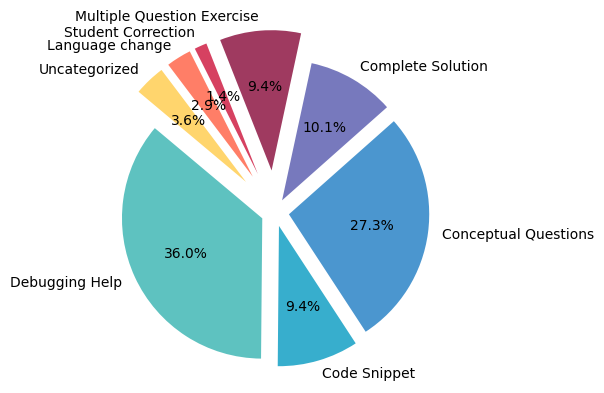
\includegraphics[scale=0.7]{figures/figure1.png}
    \caption{Classification of messages.}
    \label{fig:graph1}
\end{figure}

Approximately 64\% of the messages pertain to categories associated with
critical thinking, corroborating with the findings of
\cite{Ghimire24}. In contrast, around 28\% of the messages
indicate a preference among students for ready-made answers.

\section{Conclusion}

\bibliographystyle{IEEEtran}
\bibliography{references}

\end{document}
